For the exemplar database, we collected various face poses for 22 individuals (11 male and 11 female)
from the talk shows available online. We selected sections which have complete swing of pose and
expression changes. Approximately 15 exemplars and a frontal view were selected per individual.
In total of around 400 exemplars and 22 frontal view faces were collected. For face recognition
experiment, we collected approximately 50 training and 50 input faces of 6 celebrities online. We
call this dataset the $PoseInTheWildFaceDataSet$ (PIWFDS). We consider a new dataset, as existing
datasets do not contain profile-frontal image pairs and even state-of-the-art recognition systems
perform poorly on it.
 
 
\begin{figure}
\begin{center}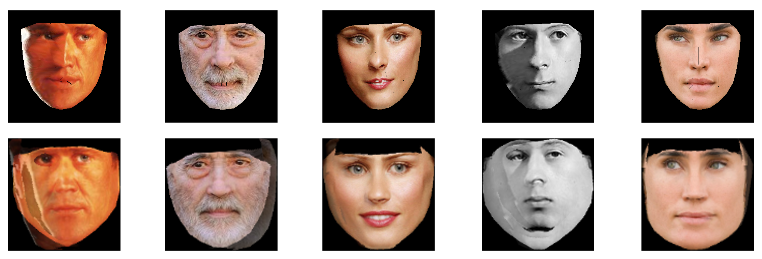
\includegraphics[width =13cm,height=5.2cm]{front/figures/qualitative_result_1.png}\end{center}
\caption{First row shows the output of our method and the second row is of Hassner {\em et al.}~\cite{DBLP:journals/corr/HassnerHPE14} for LFPW~\cite{fiducials_cvpr2011} dataset. Observe ghost like appearances, structure distortion, mirroring effects in Hassner {\em et al.}~\cite{DBLP:journals/corr/HassnerHPE14} output.}
\label{fig:qualitative_result1}
\end{figure}


All our experiments were conducted using MATLAB. We used HoG~\cite{Dalal:2005:HOG:1068507.1069007} feature based face detector to find
faces and its output is re-scaled to a $300 \times 300$ image for both the
database images and our input. This is given to facial landmark detection code
based on~\cite{kazemi2014one}, which is publicly made available. This provides 68 landmarks on each face. Using
the landmarks we divide the face surface into 110 planes (triangular in shape). Using the
corresponding planes between input profile image and the exemplar frontal view image, we compute the
homography transformations matrix using publicly available implementation of
vgg\_Haffine\_from\_x\_MLE. Using this set of homographies, we synthesize the frontal view of the input image.
